\documentclass{article}
\usepackage[utf8]{inputenc}
\usepackage{subfig}
\usepackage{amsmath}

\usepackage{graphicx}
% \usepackage[legalpaper, landscape, margin=0.5cm]{geometry}
\usepackage[legalpaper, portrait, margin=0.5cm]{geometry}

\thispagestyle{empty}
% \renewcommand{\thesubfigure}{\roman{subfigure}}
\begin{document}

\begin{figure}[h]
        \centering
        \subfloat[thickness error]{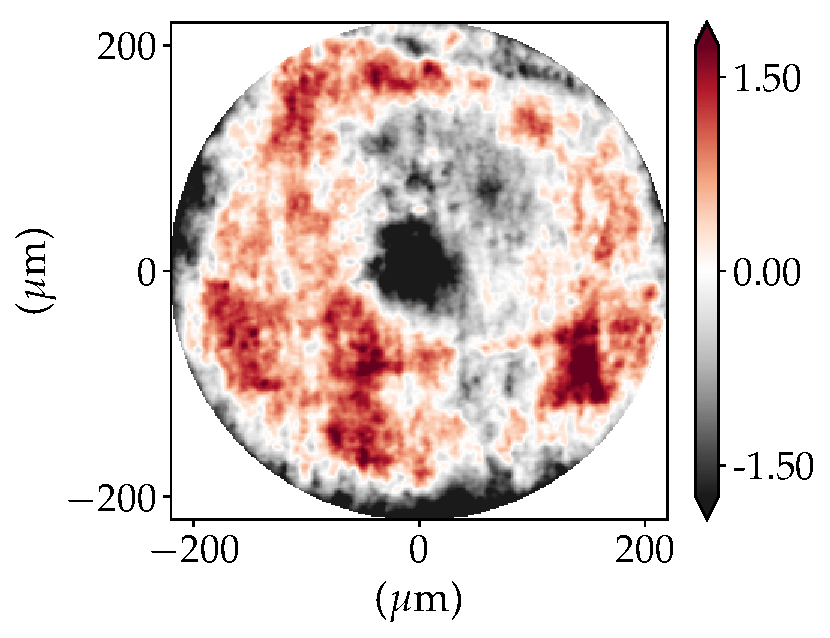
\includegraphics[height=3.5cm]{figures/ch04b/figure_errors_FF_workflow_a_FC_CDo01_these3.pdf}}\hspace{0.1cm}
        \subfloat[Zernike circle pol. fit]{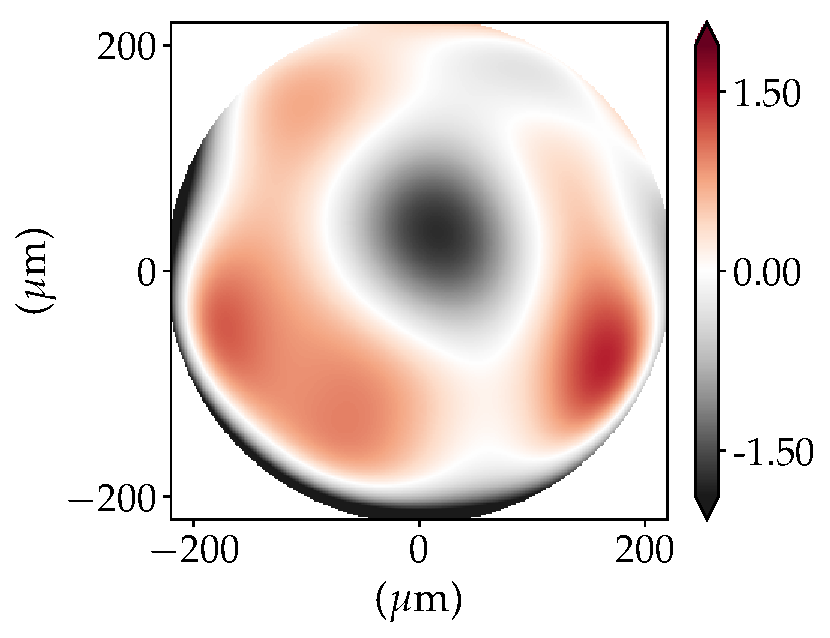
\includegraphics[height=3.5cm]{figures/ch04b/figure_errors_LF_workflow_a_FC_CDo01_these2.pdf}}\hspace{0.1cm}
        \subfloat[residues]{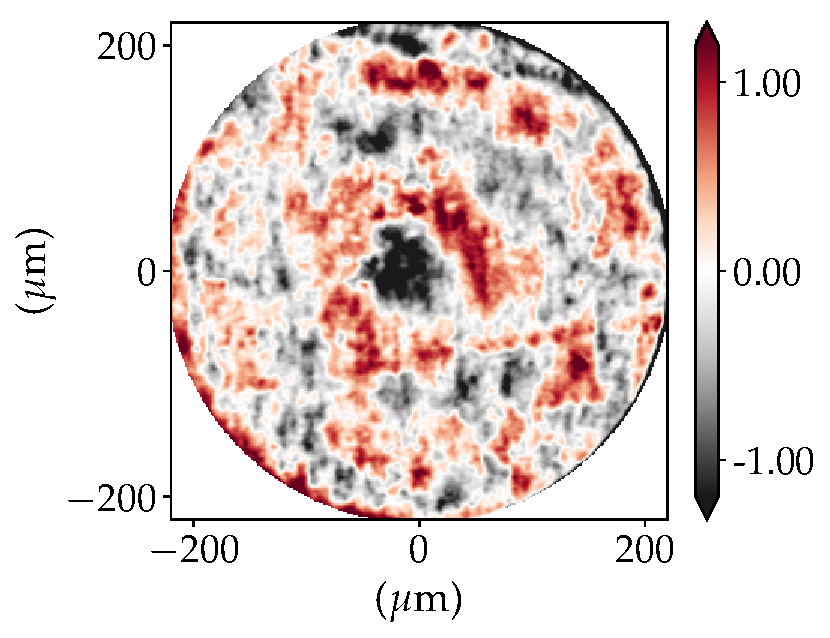
\includegraphics[height=3.5cm]{figures/ch04b/figure_errors_HF_workflow_a_FC_CDo01_these2.pdf}}\\
        \subfloat[Zernike circle polynomial fit coefficients]{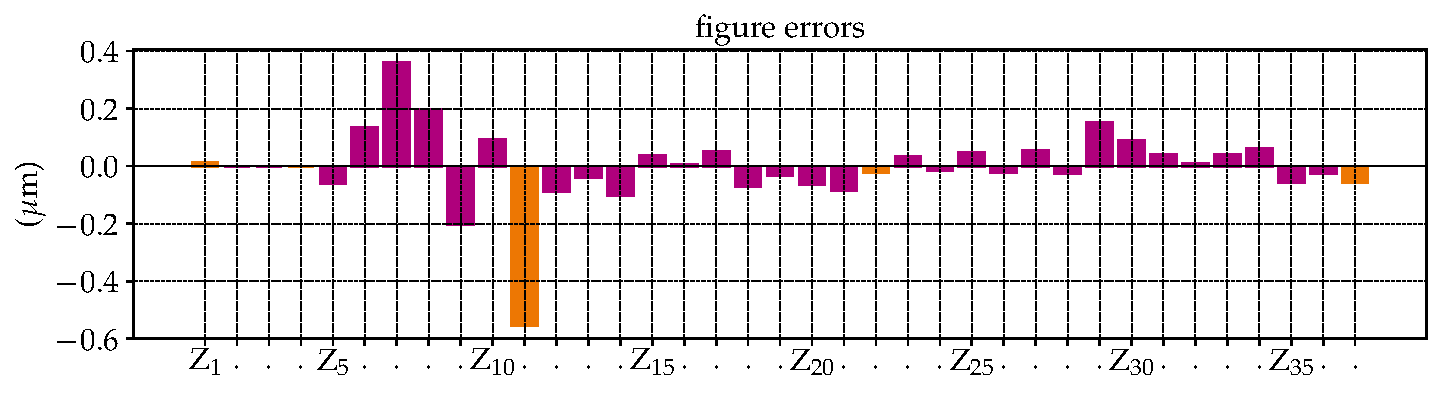
\includegraphics[height=3.8cm]{figures/ch04b/Zern_fit_workflow_a_FC_CDo01_these2.pdf}}\hspace{0.1cm}
        \subfloat[PSD]{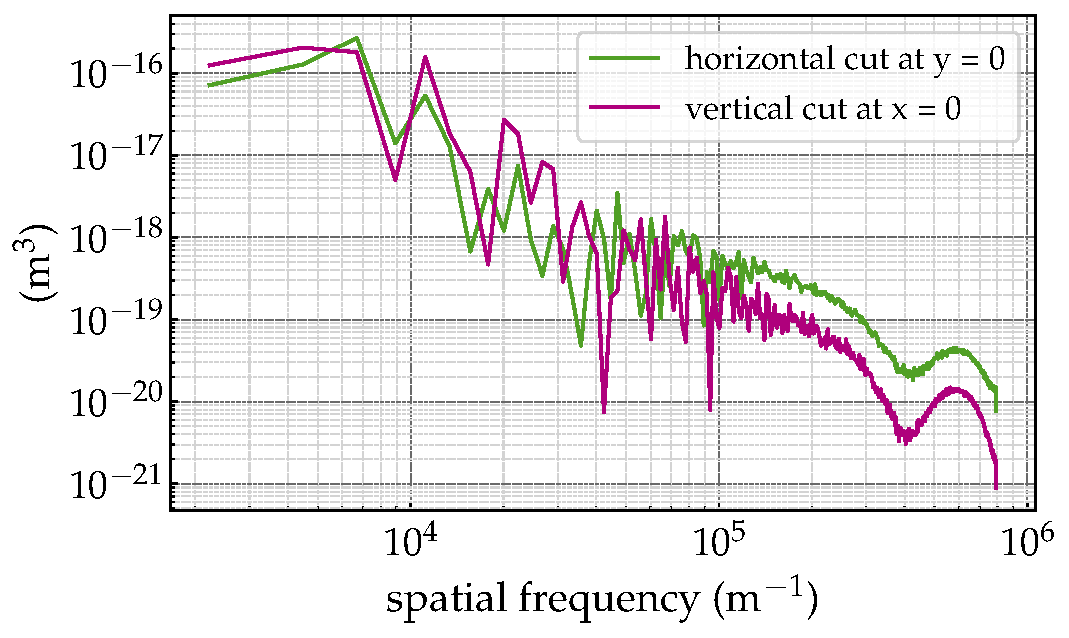
\includegraphics[height=3.92cm]{figures/ch04b/PSD_workflow_a_FC_CDo01_these2.pdf}}
 \end{figure}
\end{document}